\documentclass[10pt,b5paper,sans]{moderncv}

%% ModernCV themes
\moderncvstyle{casual}
\moderncvcolor{black}
\renewcommand{\familydefault}{\sfdefault}
\setlength{\hintscolumnwidth}{0.2\textwidth}
\nopagenumbers{}
\newcommand{\tab}{\hspace{0.3cm}}

\definecolor{blue}{rgb}{0.0,0.5,1.0}
\definecolor{orange}{rgb}{1.0,0.55,0.0}
\definecolor{green}{rgb}{0,0.8,0.25}
\definecolor{DarkOrchid}{rgb}{0.6, 0.2, 0.8}

%% Character encoding
\usepackage[utf8]{inputenc}

%% Adjust the page margins
\usepackage[inner=2.4cm,outer=2.4cm,top=2cm,bottom=3.5cm,scale=0.75]{geometry}
\usepackage{lscape}
\usepackage{pgfgantt}
\usepackage{xcolor}
%\usepackage{natbib}
\usepackage[english]{babel}
\usepackage[backend=biber,maxbibnames=99,dashed=false,style=authoryear,sorting=ydnt]{biblatex}%
\DeclareNameAlias{sortname}{last-first}
%\DeclareSortingScheme{noneyear}{
%	\sort{\citeorder}
%	\sort{\field{year}}
%}
\addbibresource{./CVbiblio.bib}
%\AfterPreamble{\hypersetup{colorlinks=false,linkbordercolor=red,pdfborderstyle={/S/U/W 1}}}

%% Personal data
\firstname{Cha\"im}
\familyname{De Mulder}
\title{}
\address{Portugalstraat 9/301}{9000 Gent}
\mobile{+32 479 74 55 02}
\email{demulderchaim@gmail.com}
%\homepage{www.johndoe.com}
\extrainfo{Born 27/3/1991 in Ghent}
\photo[76pt][0.8pt]{../images/ChaimDeMulderbis}
%\quote{Some quote (optional)}

%%------------------------------------------------------------------------------
%% Content
%%------------------------------------------------------------------------------
\begin{document}
\makecvtitle

%%%%%%%%%%%%%%%%%%%%%%%%%%%%%%%%%%%%%%%%%%%%%%%%%%%%%%%%%%%%%%%%%%%%%%%%%%%%%%
%\vspace{-0.5cm}
\colorbox{orange!10}{
	\begin{minipage}{\textwidth}
		\section{\textcolor{orange}{\textbf{Experience}}}
		\cventry{Oct. 2015 -- May 2019}{PhD Candidate}{\footnotesize Ghent University, Faculty of Bioscience engineering, Department of Data Analysis and Mathematical Modeling, BIOMATH group (Model based bioprocess analysis and optimisation)}{}{}{}
		\cvitem{\centering\raisebox{-0.7\height}{
\includegraphics[width=0.12\textwidth]{../images/LogoUGent.png}}}
		{\small Model-based decision support, knowledge build-up and advanced modeling of the Wastewater Treatment Plant of Eindhoven, The Netherlands, in close collaboration with the operators (Waterboard De Dommel).}
		\vspace{0.2cm}
		
		\cventry{Oct. 2014 -- Oct. 2015}{Research Assistant}{\footnotesize Ghent University, Faculty of Bioscience engineering, Department of Data Analysis and Mathematical Modeling, BIOMATH group (Model based bioprocess analysis and optimisation)}{}{}{}
		\cvitem{}
		{\small Hydrodynamic and biokinetic modeling in the context of the High Rate Activated Sludge process, in collaboration with Waterboard Brabantse Delta, The Netherlands}
		\vspace{0.2cm}
		
		%$\bullet$ Coupling a hydrodynamic model (using CFD) and a biokinetic model (using established wastewater treatment models) for the Wastewater Treatment Plant of Breda, The Netherlands.\newline
		%$\bullet$ Implementing a model for the simulation of the High Rate Activated Sludge Process, based on two previously described models.
		%\cventry{20/8/2014--12/11/2014}{PhD-scholarship application}{Ghent University, Faculty of Bioscience engineering, Department of Mathematical Modeling, Statistics and Bioinformatics, BIOMATH group (Model based bioprocess analysis and optimisation) and LabMET (Laboratory for Microbial and Environmental Technolgy)}{}{}{}
		%\cvitem{Project title}{Partial nitritation/anammox in mainstream: development based on hydrodynamic and kinetic modeling}
		%\cvitem{Project description}{\small Different control strategies to obtain Partial nitritation/anammox (PN/A) already exist in full-scale sidestream applications. In mainstream municipal wastewater treatment however, full-scale application has not been achieved, mainly due to hydrodynamic reactor-heterogeneity. The coupling of hydrodynamics (using CFD) and biokinetics (using established wastewater treatment models) offers a powerful way to gain insight in their interaction, and to move towards more solid design and control strategies, making full-scale PN/A implementation possible.}
		%\cvitem{\textcolor{green}{\underline{Skills}}}{Project preparation consisted of extensive literature research concerning CFD, wastewater treatment modeling, the PN/A process, the A/B-proces and multiple trial defenses}
		\cventry{2015--present}{IWA involvement}{}{}{}{}
		\cvitem{\centering\raisebox{-0.7\height}{
\includegraphics[width=0.08\textwidth]{../images/IWA}}\\}{\small 
			$\bullet$ Active YWP member in the board of directors of the Belgian branch of IWA (B-IWA)\newline
			$\bullet$ Active YWP member in the Management Committee of the IWA Specialist Group on Modeling and Integrated Assessment \newline
			%	$\circ$ Maintenance of \href{http://www.b-iwa.be}{\underline{website}}, \href{https://www.linkedin.com/groups?mostRecent=&gid=3760023&trk=my_groups-tile-flipgrp}{\underline{LinkedIn}}- and \href{https://twitter.com/BelgianIWA}{\underline{Twitter}}-account.\newline
			%$\circ$ Coordinator of the first, second and third \href{http://www.b-iwa.be/node/177}{\underline{B-IWA nocturnal}}
			$\bullet$ Organising Committee member of the IWA YWP Benelux Conference, Gent, Belgium, July 2017
		}
		\cventry{Jul. -- Aug. 2013}{Internship in combination with master thesis}{\footnotesize DC Water, Research and Development Department}{\footnotesize Washington DC, USA}{}{}
		%\cvitem{Title}{Researcher/MSc Student}
		%\cvitem{Description}{}
		%\cvitem{\textcolor{green}{\underline{Skills}}}{Operating successfully in a research working environment, team-work, critical analysis of research results}
		%\cvitem{\raisebox{-\height}{
\includegraphics[width=0.09\textwidth]{./LogoDCWater.png}}}
		%{\textbf{Project:} \small Batch experiments under different conditions to obtain AOB and NOB oxygen half-saturation constants through parameter estimation using a specific model describing the experimental procedure.}
		%\vspace{0.5cm}
		
		\cventry{Jul. -- Aug. 2012}{IAESTE Internship}{\footnotesize Aalto University, Department of Biotechnnology and Chemical Technology}{\footnotesize Espoo, Finland}{}{}
		%\cvitem{Title}{Research assistant}
		%\cvitem{\raisebox{-\height}{
\includegraphics[width=0.08\textwidth]{./LogoAalto}}}
		%{\textbf{Project:} \small Catalysts used in the dehydration of xylose to furfural were characterized using micro-scale reactors, titration experiments and sugar-adsorption measurements.}
		%\cvitem{\textcolor{green}{\underline{Skills}}}{Working independently, soft/social skills: patience, open mind, communication}
		%\vfill
		%\vspace{0.5cm}
		
		
		%\cvitem{\raisebox{-\height}{
\includegraphics[width=0.08\textwidth]{./IWA.png}}}{\small
		%	$\bullet$ Co-organizer of an \href{http://www.iwarr2015.org/content/young-professionals-workshop-building-pipelines-resource-recovery}{\underline{IWA YWP Workshop}} (Aug 29 - 30, 2015)\newline
		%	$\bullet$ Assistant in the course Modeling and Control of Wastewater Treatment Plants, given at the Faculty of Bioscience Engineering, Ghent University.}
		
	%	\vspace{0.5cm}
	\end{minipage}
}

%%%%%%%%%%%%%%%%%%%%%%%%%%%%%%%%%%%%%%%%%%%%%%%%%%%%%%%%%%%%%%%%%%%%%%%%%%%%%%
\colorbox{blue!10}{
	\begin{minipage}[]{\textwidth}
		\section{\textcolor{blue}{\textbf{Education}}}
		\cvitem{}{Ghent University}
		%\cventry{2014--present}{PhD in Bio-Science Engineering: 	Environmental Technology}{Ghent University}{}{}{}
		\cventry{2012--2014}{Master in Bio-Science Engineering: Environmental Technology}{}{}{}{}
		%\cvitem{}{\textbf{MSc Thesis:} Impact of intrinsic and extrinsic parameters on the oxygen kinetic parameters of Ammonia and Nitrite Oxidizing Bacteria}
		%\cvitem{University}{Ghent University}
		%\cvitem{}{\textbf{Research group:} LabMET (Laboratory for Microbial and Environmental Technolgy) \& BIOMATH (Model-based Bioprocess Analysis and Optimisation)}
		%\cvitem{}{\textbf{Abstract:}\\ \small Batch experiments were conducted under different conditions to obtain AOB and NOB oxygen half-saturation constants through parameter estimation using a specific model describing experimental procedure. Using the obtained values, relations that indicate conditions under which AOB would outcompete NOB were sought for, making energy-efficient N-removal through anammox possible.}
		%Using the obtained values, relations that indicate conditions under which AOB would outcompete NOB were sought for, potentially making energy-efficient N-removal through the anammox process possible.
		\cventry{2009--2012}{Bachelor in Bio-Science Engineering: Environmental Technology}{}{}{}{} 
	%	\cvitem{}{\textbf{BSc Thesis:} Integrated grey water systems in city renovation and development projects}
		%\cvitem{University}{Ghent University}
		%\cvitem{}{\textbf{Department:} Biosystems engineering }
		%\cvitem{}{\textbf{Abstract:}\\ \small Batch experiments were conducted under different conditions to obtain AOB and NOB oxygen half-saturation constants through parameter estimation using a specific model describing experimental procedure. Using the obtained values, relations that indicate conditions under which AOB would outcompete NOB were sought for, making energy-efficient N-removal through anammox possible.}
		
		%\cventry{2003--2009}{Secondary school degree}{OLV-College Campus Bevegem, Zottegem}{}{}{Latin-Mathematics}  % arguments 3 to 6 can be left empty
		%\cvitem{title}{ \emph{Title} }
		%\cvitemwithcomment{Language 1}{Skill level}{Comment}
		%\cvdoubleitem{category X}{XXX, YYY, ZZZ}{category Y}{XXX, YYY, ZZZ}
		%\cvlistitem{Item 1}
		%\cvlistdoubleitem{Item 2}{Item 3}
		%% ...
	\end{minipage}
}
%%%%%%%%%%%%%%%%%%%%%%%%%%%%%%%%%%%%%%%%%%%%%%%%%%%%%%%%%%%%%%%%%%%%%%%%%%%%%%
\vfill
\colorbox{green!10}{
	\begin{minipage}{\textwidth}
		\section{\textcolor{green}{\textbf{Extra-curricular}}}
		\cventry{2018--present}{\href{http://climate-express.be}{\textbf{Climate Express}}}{}{}{}{}
		\cvitem{\centering\raisebox{-0.4\height}{
\includegraphics[width=0.05\textwidth]{../images/ClimateExpress}}\\}{Voluteering and campaining for a socially just transition to a carbon-neutral society.}
		\cventry{2018--present}{\href{https://www.climateresponse.eu}{\textbf{Climate Response}}}{}{}{}{}
		\cvitem{\centering\raisebox{-0.2\height}{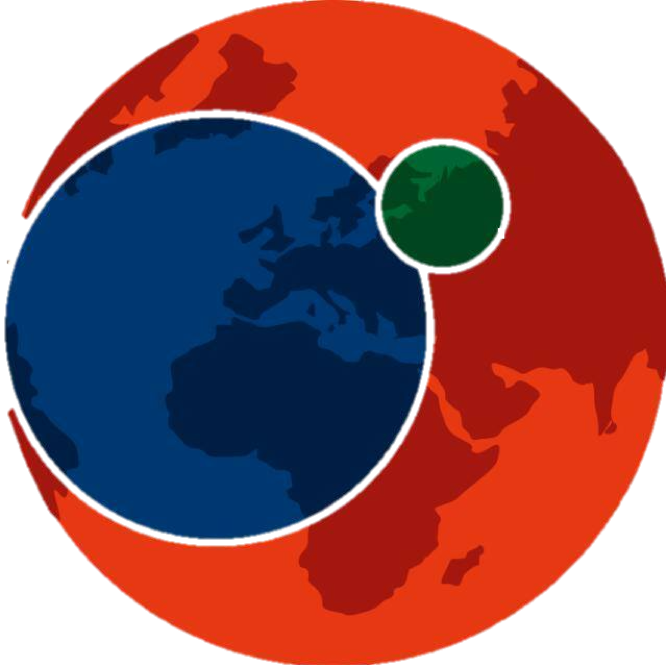
\includegraphics[width=0.05\textwidth]{../images/ClimateResponse}}\\}{Spreading facts on Climate Change in order to spread the urgent message that societal change is required to tackle the problem.}
		\cventry{2018--present}{\href{https://www.yaku.be}{\textbf{YAKU}}}{}{}{}{}
		\cvitem{\centering\raisebox{-0.2\height}{
\includegraphics[width=0.05\textwidth]{../images/yaku.png}}\\}{Citizen science with the ultimate goal to make swimming in the open waters of Ghent possible.}
		\cventry{2013--2018}{\href{https://iaeste.org}{\textbf{IAESTE}}}{}{}{}{}
		\cvitem{\centering\raisebox{-0.5\height}{
\includegraphics[width=0.05\textwidth]{../images/iaeste_logo}}\\}{International Association for the Exchange of Students for Technical Experience, arranging internships for technical students for over 70 years.}
		%\cvitem{2017--2018}{\textbf{Connect Region Project Coordinator}}
		%: \small Member of the Regional Management team of western Europe, day-to-day manamement of regional affairs. Responsible for several projects with participants from across the region.
		%\cvitem{}{ \normalsize}
		%\cvitem{2016--2017}{\textbf{LC Ghent Exchange Coordinator}}
		%: \small Board member of the Local Committee of Ghent, day-to-day management of a 25-person team of students. Resposible for international internship exchange and networking, jobraising.
	    %\cvitem{}{ \normalsize}
		%\cvitem{2015--2016}{\textbf{LC Ghent Vice-President \& Summer Reception Officer}}
		%\cvitem{}{\normalsize}
		%: \small General support on local level (team management)  and within international IAESTE groups (Region of western Europe). Jobraising and organizing activities for incoming trainees.
		%\cvitem{2014--2015}{\textbf{LC Ghent supporting member \& Summer Reception Officer}}
		%: \small Design of PR materials, presenting IAESTE to companies, jobraising. Organizing activities for incoming trainees. 
		%\cvitem{}{\normalsize}
		%\cvitem{2013--2014}{\textbf{LC Ghent Secretary}}
		%: \small Responsible for meeting reports, jobraising. 
		%\cvitem{}{\normalsize}
		%\vspace{0.5cm}
		\cvitem{}{\textbf{Sports and general interests}}
		\cvitem{}{Athletics (recreational and competition), music, board games, climate related, environmental and social issues, Nordic culture.}
		%\cvitem{}{\textbf{General interests}}
		%\cvitem{}{Music, climate related, environmental and social issues, Scandinavian culture}
		%\cvitem{}{Open Source initiatives}
		%\cvitem{}{Climate related and environmental issues}
	\end{minipage}
}
\vfill

%%%%%%%%%%%%%%%%%%%%%%%%%%%%%%%%%%%%%%%%%%%%%%%%%%%%%%%%%%%%%%%%%%%%%%%%%%%%%%
\colorbox{DarkOrchid!10}{
	\begin{minipage}{\textwidth}
		\section{\textcolor{DarkOrchid}{\textbf{Skills}}}
		\cvitem{}{Motivated environmental engineer with good analytic skills and a broad interest range; my major motivators are climate and environmentally related issues.}
		%\vspace{-.55cm}
		%\cvlistitem{Social och \textbf{storsint}}
		%\cvlistitem{Team-worker}
		\cvitem{}{Focus on efficiency, structure and clear communication, both in individual and team work.}%, och d\"arf\"or ocks\aa\ van vid bra \textbf{time management}.}
		%\cvitem{}{$\bullet$ Grundl\"aggande kunskaper inom \textbf{project management}.}
		\cvitem{}{Social and open minded}
		\vspace{0.2cm}		
		\cvitem{Software/IT}{$\bullet$ Advanced: Python, \LaTeX, WEST}
		%\vspace{-.55cm}
		\cvitem{}{$\bullet$ Basic: MS Office, Inkscape, Drupal}
		%OpenFOAM, git(hub)
		\vspace{0.2cm}
		\cvitem{Languages}{
			\begin{tabular}{ll}
				$\bullet$ Dutch (native) & \tab $\bullet$ English (fluent)\\
				$\bullet$ Swedish (advanced) & \tab $\bullet$ French (basic)\\	
		\end{tabular}}
	\end{minipage}
}
\vfill
%%%%%%%%%%%%%%%%%%%%%%%%%%%%%%%%%%%%%%%%%%%%%%%%%%%%%%%%%%%%%%%%%%%%%%%%%%%%%%
\begin{center}
	\begin{ganttchart}[
		%hgrid=true,
		%vgrid=true,
		y unit title=0.8cm,
		y unit chart=0.5cm,
		x unit=0.6cm,
		bar1/.style={bar/.append style={fill=blue}},
		bar2/.style={bar/.append style={fill=orange}},
		bar3/.style={bar/.append style={fill=green}},
		bar4/.style={bar/.append style={fill=DarkOrchid}}
		]{1}{16}
		\scriptsize
		\ganttset{group height=0.5cm}
		\gantttitle{2012}{2} \gantttitle{2013}{2} \gantttitle{2014}{2} \gantttitle{2015}{2} \gantttitle{2016}{2}\gantttitle{2017}{2}\gantttitle{2018}{2}\gantttitle{2019}{2}\\
		\textcolor{blue}{\ganttbar[bar1]{Masters Degree}{1}{5}}\\
		\textcolor{orange}{\ganttbar[bar2]{IAESTE Internship}{2}{2}}\\
		\textcolor{orange}{\ganttbar[bar2]{DC Water Internship}{4}{4}}\\
		\textcolor{orange}{\ganttbar[bar2]{Research Assistant}{6}{7}}\\
		\textcolor{orange}{\ganttbar[bar2]{PhD Candidate}{8}{15}}\\
		\textcolor{orange}{\ganttbar[bar2]{IWA Involvement}{7}{15}}\\
		\textcolor{green}{\ganttbar[bar3]{IAESTE Member}{3}{13}}\\
		\textcolor{green}{\ganttbar[bar3]{Climate Response}{14}{15}}\\
		\textcolor{green}{\ganttbar[bar3]{Climate Express}{14}{15}}\\
		\textcolor{green}{\ganttbar[bar3]{YAKU}{14}{15}}\\
		%\textcolor{green}{\ganttbar[bar3]{IAESTE support}{14}{16}}\\
		%\textcolor{green}{\ganttbar[bar3]{IAESTE Vice President}{14}{16}}\\		
		\textcolor{green}{\ganttbar[bar3]{Athletics}{1}{15}}\\
		\textcolor{DarkOrchid}{\ganttbar[bar4]{Swedish classes}{6}{15}}
		\normalsize
	\end{ganttchart}
\end{center}
\vfill
\newpage

%%%%%%%%%%%%%%%%%%%%%%%%%%%%%%%%%%%%%%%%%%%%%%%%%%%%%%%%%%%%%%%%%%%%%%%%%%%%%%
%\section{Personal}
%\cvitem{}{I am a \textbf{motivated and enthusiastic} young man, looking for a \textbf{challenging and diversified} job. During both my working experiences so far, I found that contact with colleagues is something I really appreciate. I am convinced that \textbf{working in a team} with people of different backgrounds can yield better results and more creative engineering solutions.\newline Since I believe I have \textbf{strong values}, I am looking for an employer whose vision I can easily identify with. It goes without saying that I will be even more eager to show a \textbf{committed engagement} working for a company that appeals to me.}

%Obviously, I am ready to show a \textbf{commited engagement} in such a context. }
%\cvitem{Looking for}{Challenging and diversified job, team-work, employer vision and mission I can identify with}
%%%%%%%%%%%%%%%%%%%%%%%%%%%%%%%%%%%%%%%%%%%%%%%%%%%%%%%%%%%%%%%%%%%%%%%%%%%%%%
%\section{Attended meetings and conferences}
%\cvitem{}{\textbf{EU COST-Action meeting}, \textit{Paris}, /3-/4/2015: represent the research group professor in working group on modeling for decision support.}
%\cvitem{}{\textbf{Resource Recovery Conference 2015},\textit{Gent}, /9/2015-/9/2015}
%\cvitem{}{\textbf{IAESTE Annual Conference},\textit{Prague}, 22/1/2016-29/1/2016}


%%%%%%%%%%%%%%%%%%%%%%%%%%%%%%%%%%%%%%%%%%%%%%%%%%%%%%%%%%%%%%%%%%%%%%%%%%%%%%
\section{\textbf{Scientific publications}}
%\renewcommand{\section}[2]{}
%\subsection{Journal papers}
\nocite{*}
\printbibliography[type=article,title={Journal papers}]
\newpage
\printbibliography[type=inproceedings,title={Conference papers (presentations and posters)}]%,sorting=noneyear]
\printbibliography[type=manual,title={Software}]%,sorting=noneyear]
\newpage
\section{\textbf{Scientific conferences}}
\cvitem{{\centering Apr. 2--6, 2016}}{IWA/WEF Wastewater Treatment Plant Modeling seminar (WWTMod)\newline Annecy, France, Workshop co-organizer}

\cvitem{May 21--24, 2017}{Frontiers International Conference on Wastewater Treatment (FICWTM) \newline Palermo, Italy, Oral presentation}

\cvitem{June 11--14, 2017}{IWA Specialized Conference on Instrumentation, Control and Automation (ICA) \newline Qu\'ebec City, Canada, Oral presentation (not present at the conference)}

\cvitem{July 5--7, 2017}{Young Water Professionals BeNeLux conference \newline Ghent, Belgium, Oral presentation}

\cvitem{Nov. 7--9, 2017}{IWA Conference on sustainable Wastewater Treatment and Resource Recovery: Research, Planning, Design and Operation (NRR-LWWTP)\newline Chongqing, China, Oral presentation}

\cvitem{Mar. 10--14, 2018}{IWA/WEF Water Resource Recovery Modelling Seminar (WRRMod)\newline Qu\'ebec City, Canada, Poster presentation}

\cvitem{Sept. 16--21, 2018}{IWA World Water Congress and Exhibition\newline Tokyo, Japan, Poster presentation (not present at the conference)}

\cvitem{June. 10--14, 2019}{IWA Leading Edge Technologies Conference (IWA-LET)\newline Edinburgh, United Kingdom, Poster presentation (not present at the conference)}

\cvitem{September. 1--4, 2019}{IWA Symposium on Modeling and Integrated Assessment (Watermatex)\newline Kopenhagen, Denmark, Oral presentation (not present at the conference)}

\section{\textbf{Educational activities}}
\cvitem{Teaching}{
	$\bullet$ Assisting with the Master course Modeling and Control of Wastewater Treatment Plants
}{}{}{}{}
\cvitem{MSc students tutored}{
	$\bullet$ Katrien Couchez: Modeling the effect of urine separation on full-scale Waste Water Treatment Plant operation.\newline
	$\bullet$ Vincent Van De Maele: The impact of fluctuating energy prices on WWTP cost optimisation\newline
	$\bullet$ Tom Lauriks: Opportunities and limitations of connecting Life Cycle Assessment to a dynamic wastewater treatment plant model
}{}{}{}{}
\cvitem{Internship students (co-)tutored}{
	$\bullet$ Tamare K\"unzle: development of the \textit{wwdata} package and model calibration of the B\"urger-Diehl settler model. \newline
	$\bullet$ Jora Singh Randhawa: development of the \textit{wwdata} python package.\newline
	$\bullet$ Attilio Di Nisio: development of a model of the Cuiodepur WWTP
}{}{}{}{}

\end{document}